\chapter{Derivation of the line-source equation}
\label{app:linesource}
\index{Line source approximation}
We here present the derivation of the line source equation.
This derivation closely mimics Appendix C in \citeasnoun**{Holt1998}.
We start with the point-source equation (Equation \ref{eq:VC:pointsource2})
\begin{equation}
\phi_k({\bf r}, t) = \frac{I_k}{4\pi \sigma_t |{\bf r-r_k}|}.
\end{equation}
We integrate this equation along the segment,
\begin{equation}
\phi_k({\bf r},t) = \frac{I_k}{4\pi \sigma_t} \int \frac{dr_k}{|{\bf r-r_k}|} = 
\frac{I_k}{4\pi \sigma_t \Delta s_k} \log \left| \frac{\sqrt{h_k^2+\rho_k^2}-h_k}{\sqrt{\ell_k^2+\rho_k^2}-\ell_k} \right|.
\end{equation}
\tvnnote{This derivation should be expanded}
\begin{figure}[!ht]
\begin{center}
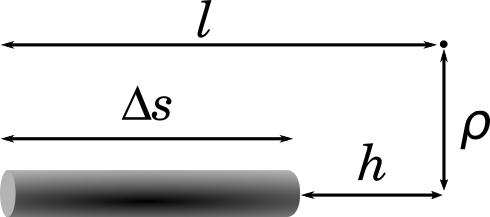
\includegraphics[width=0.5\textwidth]{Figures/VC/line_source_illustration.png}
\end{center}
\caption[]{\textbf{Line-source approximation.} Definitions of symbols used in the line-source approximation. }
\label{App:fig:line_source_illustration}
\end{figure}
